\section{速度特性}

\subsection{飞行包线与几个特征速度}

\subsubsection{飞行包线的确定}

在前节中,
已经在一些简化情形下,
将可用推力$T_a$(分为加力和不加力)运用样条插值方法、
以及对需用推力$T_R$运用$C_L-C_D$极曲线拟合关系,
将$T_a$和$T_R$归结为巡航高度$h$和飞行马赫数$Ma$的函数:
\begin{equation}
    \begin{cases}
        \begin{aligned}
            T_a & = T_a(h,Ma)\\
            T_R & = T_R(h,Ma)
        \end{aligned}
    \end{cases}
\end{equation}

于是在给定的巡航高度$h=h^*$的情况下,
在某飞行马赫数下会有:
\begin{equation}
    T_a(h^*,Ma) = T_R(h^*,Ma)
\end{equation}

根据前节图\ref{不同高度下可用推力与需用推力与飞行马赫数的关系}中,
一般$T_a$和$T_R$会有两个交点(在$T_a$外插的情况下),因此在巡航高度$h^*$上,
可以根据交点求出两个飞行马赫数$Ma$。
其中较小的为$Ma_{\min}$,较大的为$Ma_{\max}$,
这表示在高度$h^*$时的巡航马赫数范围。
如图\ref{某高度巡航下飞行马赫数范围的确定}所示为该巡航马赫数范围确定的方法。

\subsubsection{有利飞行马赫数$M_{opt}$的确定}

在给定高度上存在一个有利飞行马赫数$Ma_{opt}$,
此飞行马赫数下会使得需用推力$T_R$取得最小值,
即需用推力最小。
\begin{equation}
    T_{R.\min}(h^*) = T_R(h^*, Ma_{opt})
\end{equation}

如图\ref{某高度巡航下飞行马赫数范围的确定}中$M_{opt}$对应于需用推力最小值$T_{R.\min}$。

\subsubsection{陡升飞行马赫数$M_{\gamma}$的确定}

在上升飞行的计算中,假定可用推力全部使用,
可以得到上升角:
\begin{equation}
    T_a=T_R+W\sin\gamma\rightarrow \gamma=\arcsin \frac{T_a - T_R}{W}
\end{equation}

假设飞行中飞行器质量不变(即极短的一个任务剖面),
在飞行马赫数范围$[Ma_{\min},Ma_{\max}]$之间,
必然存在一个使得剩余推力$\Delta T$使得$T_a$与$T_R$差值最大,
其中剩余推力定义为:
\begin{equation}
    \Delta T = T_a(h^*,Ma) - T_R(h^*,Ma)
\end{equation}

在此高度上,使得剩余推力$\Delta T$取最大值的飞行马赫数称为$Ma$陡升飞行马赫数,
记作$Ma_{\gamma}$,
此时上升角$\gamma$能取得最大值,
对于特定高度上,该陡升飞行马赫数是唯一确定的。
\begin{equation}
    \Delta T_{\min}(h^*) = \Delta T(h^*, Ma_{\gamma})
\end{equation}

如图\ref{某高度巡航下飞行马赫数范围的确定}中$M_{\gamma}$中所示对应于$\Delta T_{\max}$。

\begin{figure}[H]
    \centering
    \begin{tikzpicture}
        \node at (10, -0.5) {$Ma$};
        \node at (-0.5, 5) {$T$};
        \node at (8, 3.3) {$T_R$};
        \node at (4, 2.5) {$T_a$};

        \draw[->] (0, 0)--(10, 0);
        \draw[->] (0, 0)--(0, 5);
        \draw[domain=0:9, smooth] plot(\x, {(\x-4)^4/200 + (\x-4)^2/50 +1});
        
        \draw[domain=0:10, smooth] plot(\x, { 0.2*\x +1});
        \draw[dashed] (1.533, 0)--(1.533, 1.306);
        \draw[dashed] (8, 0)--(8, 2.6);
        \node at (1.533, -0.5) {$Ma_{\min}$};
        \node at (8, -0.5) {$Ma_{\max}$};

        \draw[<->, line width=2pt] (5.848, 1.127)--(5.843, 2.169);
        \node at (6.5, 1.8) {$\Delta T_{\max}$};

        \draw[dashed] (5.848, 0)--(5.848, 1.127);
        \node at (5.848, -0.5) {$M_{\gamma}$};
        \draw[dashed] (4, 0)--(4, 1);
        \node at (4, -0.5) {$M_{opt}$};
        \node at (4.6, 0.5) {$T_{R.\min}$};

    \end{tikzpicture}
    \caption{某高度巡航下飞行马赫数范围及特征马赫数的确定}
    \label{某高度巡航下飞行马赫数范围的确定}
\end{figure}

\subsubsection{飞行包线的绘制}

在前述流程明确后,
对于飞行马赫数范围需要在各个高度上求两个隐式函数相减$T_a-T_R=0$的零点(求根问题)。
对于有利飞行马赫数与陡升飞行马赫数,
则需要求取某个隐式函数的极值点(优化问题)。
对于求根问题可以用二分法求解,
优化问题也可以遍历区域搜索,
得到工程可用的数值解。
本次作业对于求根问题采用Roots.jl包,
优化问题采用Optim.jl包进行处理。

通过样条插值、函数定义、接口调用后,
可以求得不同高度$h$上对应的飞行马赫数范围、有利飞行马赫数和陡升飞行马赫数,
再次用样条插值,
将其绘制在一张图中,
得到飞行包线图如\ref{飞行包线图}所示。

\begin{figure}[H]
    \centering
    \subfloat[$Ma$]{
        \label{envelope Ma}
        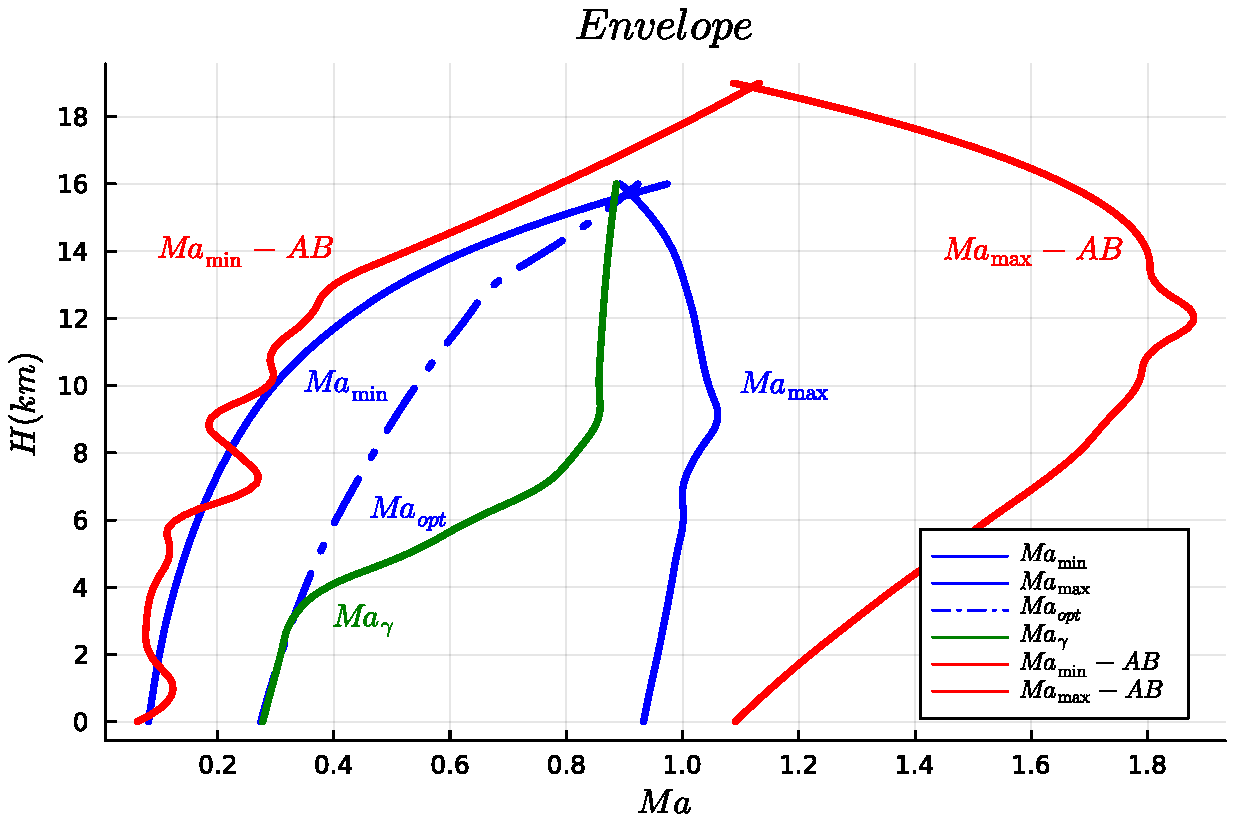
\includegraphics[width=0.5\textwidth]{image/ch5/envelope.pdf}
    }
    \subfloat[$V$]{
        \label{envelope V}
        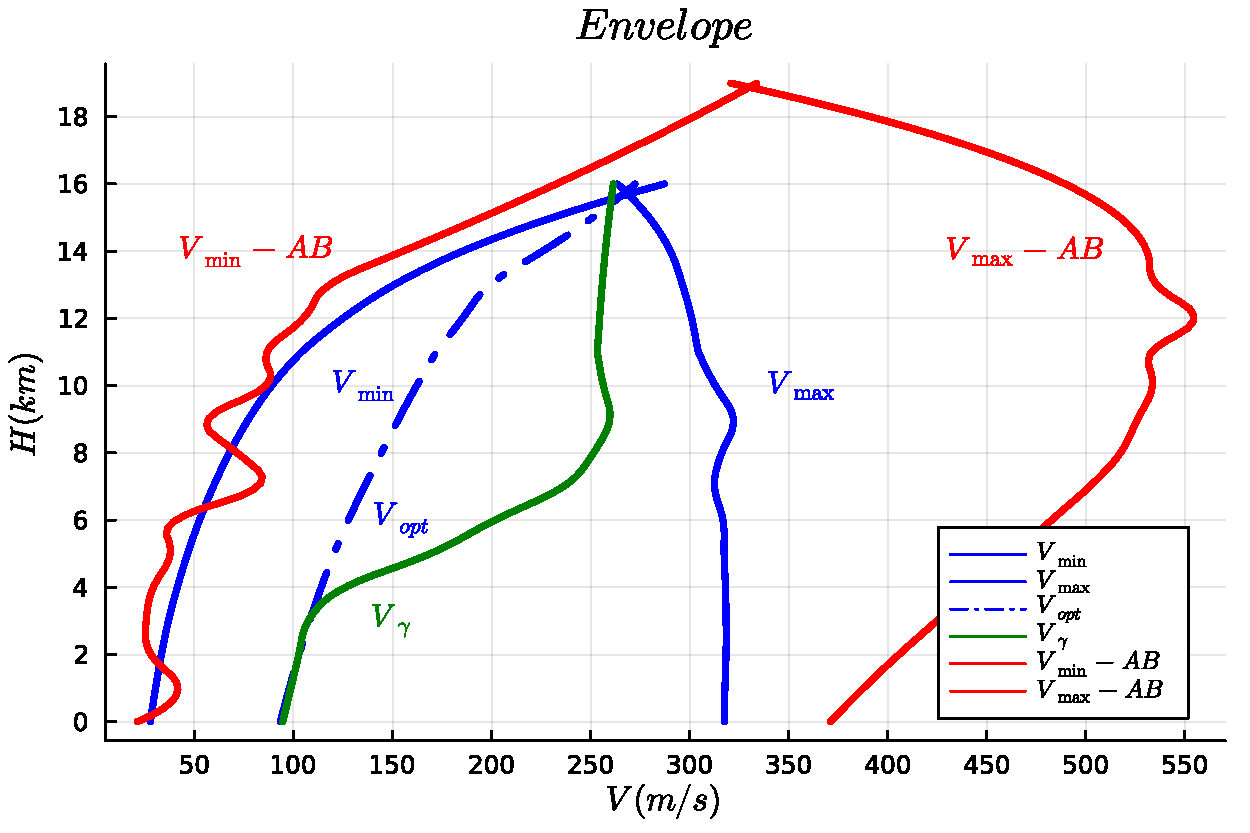
\includegraphics[width=0.5\textwidth]{image/ch5/envelope_V.pdf}
    }
    \caption{飞行包线图}
    \label{飞行包线图}
\end{figure}

其中图\ref{envelope Ma}为马赫数表示,
\ref{envelope V}为真实速度表示($V=Ma\cdot c$)。
横坐标为速度(马赫数或者速度),
纵坐标为巡航高度,
其中蓝色实线表示不加力情形下的飞行马赫数范围$Ma_{\min}$与$Ma_{\max}$,
蓝色点划线表示有利飞行马赫数$Ma_{opt}$;
红色实线表示加力情形下的飞行马赫数范围$Ma_{\min}-AB$与$Ma_{\max}-AB$;
绿色实线表示陡升马赫数$M_{\gamma}$,
左侧为第二平飞范围,
右侧为第一平飞范围。

在图中可以发现在高度大概为$15km$的时候,蓝色实线相交,
这表示不加力情况下的升限;
红色实线在约$19km$处相交,
这表示加力情况下的升限;
绿色实线与蓝色虚线在低空处一致,
即$Ma_{\gamma}\approx Ma_{opt}$,
这可以理解为不加力情形下的可用推力$T_a$在高空时,对巡航高度变化更为敏感。

\subsection{上升率$V_v$特性}

\subsubsection{上升率$V_v$的推导}

上升率是指飞机以特定的重量和给定发动机工作状态进行定常上升时在单位时间内上
升的高度,也称上升垂直速度,如图\ref{上升率Vv图示}中,
可以表示为:
\begin{equation}
    V_v = \frac{dH}{dt} = V\sin\gamma
\end{equation}


\begin{figure}[H]
    \centering
    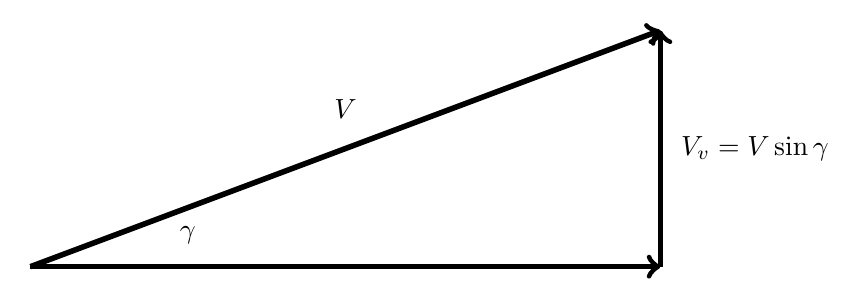
\begin{tikzpicture}
        \draw[->, line width=2pt](0, 0)--(8, 0);
        \draw[->, line width=2pt](8, 0)--(8, 3);
        \draw[->, line width=2pt](0, 0)--(8, 3);

        \node at (2, 0.4) {$\gamma$};
        \node at (4, 2) {$V$};
        \node at (9.2, 1.5) {$V_v=V\sin\gamma$}; 
    \end{tikzpicture}
    \caption{上升率$V_v$图示}
    \label{上升率Vv图示}
\end{figure}
代入上升角$\gamma$的公式,并且认为$\gamma$角极小,有$\gamma\approx \sin\gamma$。
于是可以计算得到飞行器的上升率$V_v$:
\begin{equation}
    V_v=\frac{\Delta T V}{W}= SEP = \left( \frac{T_a}{W} - \frac{1}{K} \right)V
\end{equation}

因为$\Delta T$是巡航高度和飞行马赫数的函数,而$V=Ma c$也为巡航高度和飞行马赫数的函数,
因此在给定高度$h^*$上飞行时,
组合参数$\Delta T \cdot V$可以在某一马赫数$Ma$下取得最大值,假定飞行器质量不变,
则此时能获得$V_{v.\max}$,则此时对应的飞行马赫数称作快升马赫数$Ma_{qc}$,
一般来讲快升速度$V_{qc}$略大于陡升速度$V_{\gamma}$。
快升马赫数满足:
\begin{equation}
    \begin{aligned}
        [\Delta T V(h^*,Ma)]_{\max} &= \Delta T V(h^*,Ma_{qc})\\
        V_{v.\max}(h^*) &= V_v(h^*, Ma_{qc})
    \end{aligned}
\end{equation}

\subsubsection{不同高度的上升率曲线}

在上述$V_v$的推导下,
给定巡航高度和飞行马赫数下的$V_v$可以用$(T_a-T_R)/W$表示,
在给定高度上,
可以绘制$V_v-Ma$的函数曲线。
因为线条较多较杂,
本次作业每隔$2km$为高度作出$V_v-Ma$在不同高度上的曲线关系族。

\begin{figure}[H]
    \centering
    \subfloat[不加力状态]{
        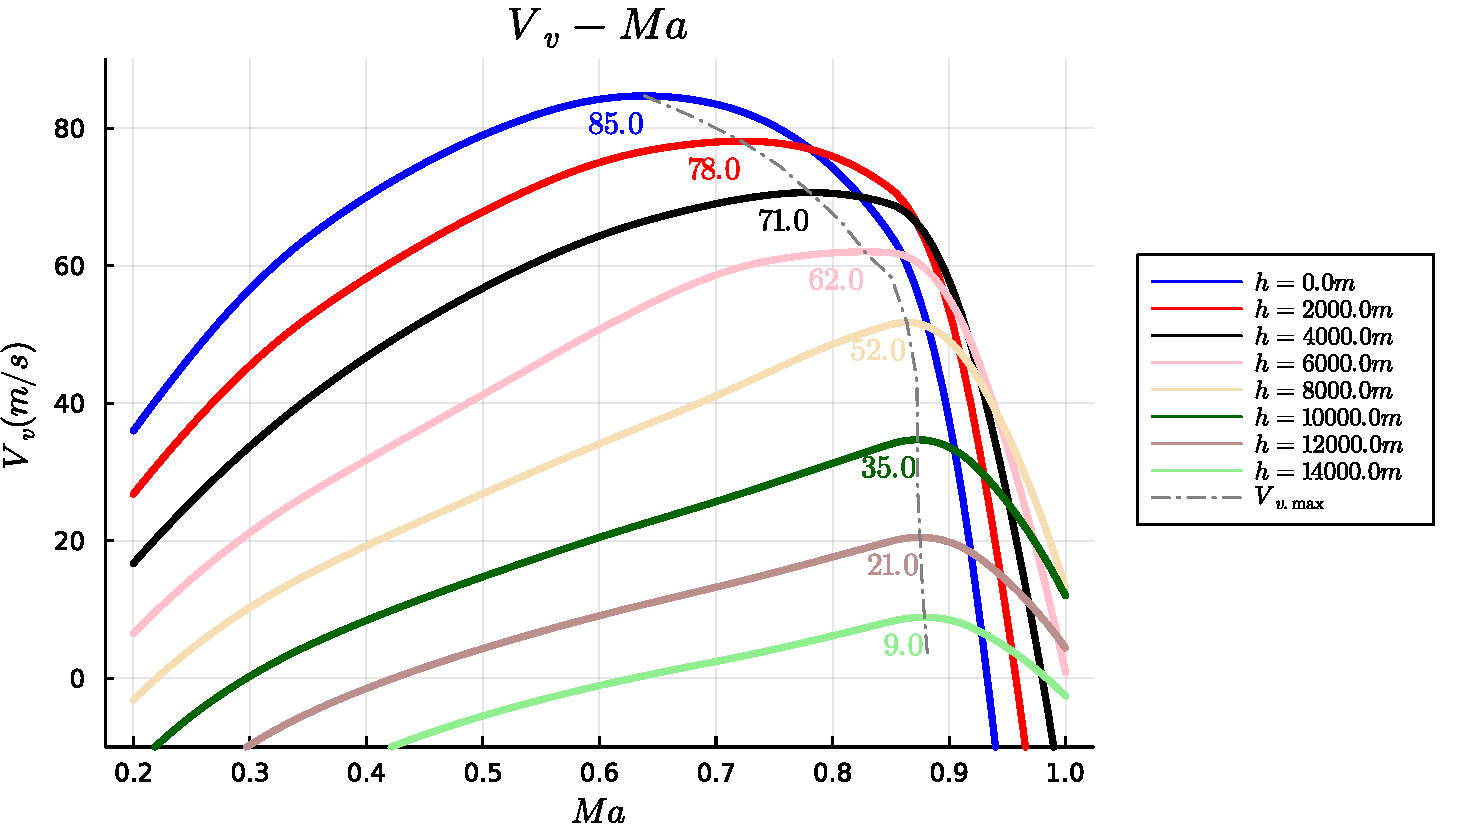
\includegraphics[width=0.5\textwidth]{image/ch5/Vv_at_all_h.pdf}
    }
    \subfloat[加力状态]{
        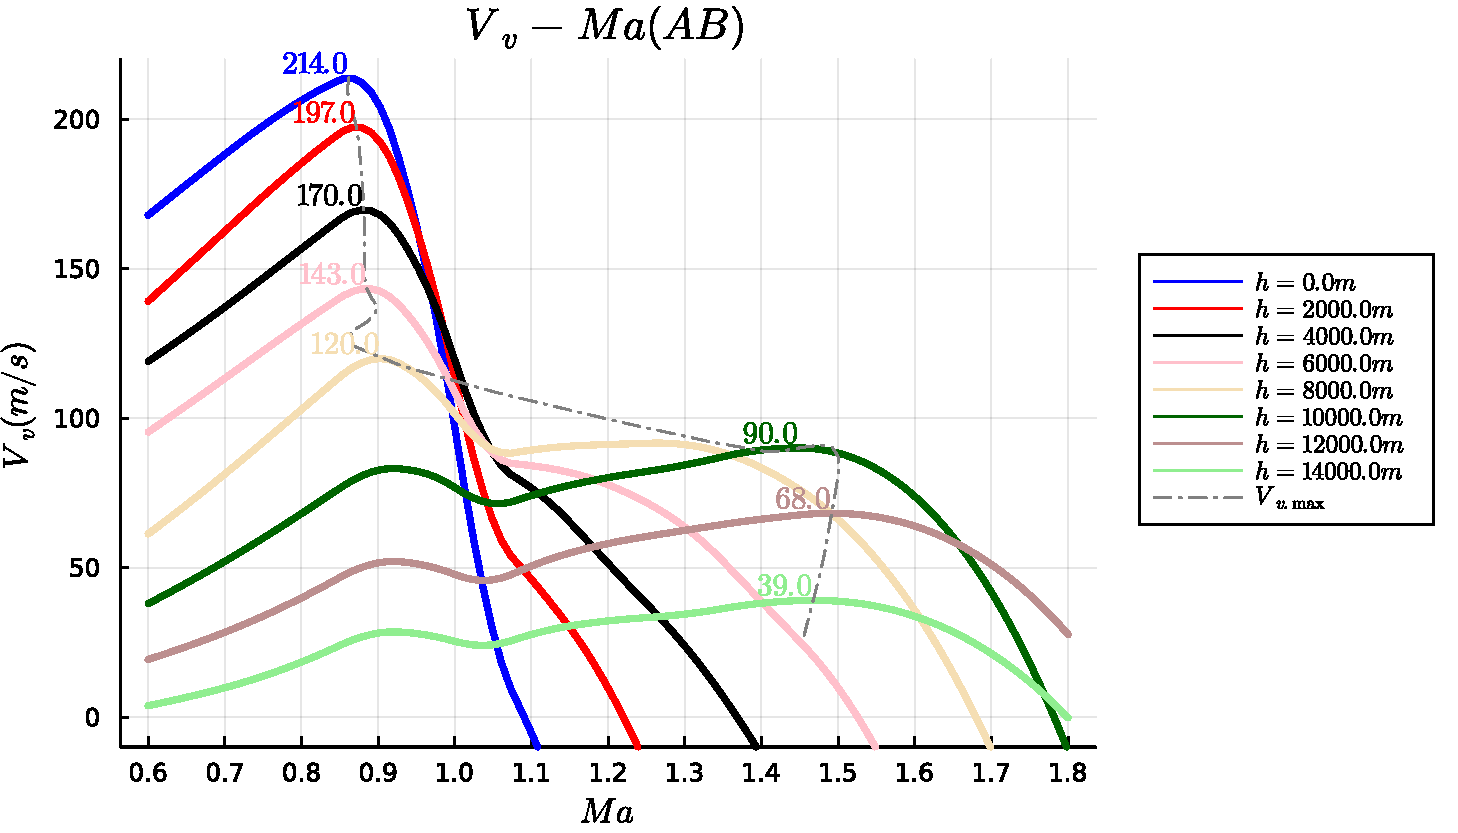
\includegraphics[width=0.5\textwidth]{image/ch5/VvAB_at_all_h.pdf}
    }
    \caption{不同高度下飞行马赫数$Ma$与上升率$V_v$曲线族}
    \label{不同高度下飞行马赫数与上升率曲线族}
\end{figure}

图\ref{不同高度下飞行马赫数与上升率曲线族}分别为加力与不加力状态下的马赫数与上升率曲线关系,
很显然随着高度升高,
整个曲线趋于“垮塌”向$Ma$轴的趋势,
这表明巡航高度越高,
剩余推力越小。
同时灰色虚线标明了各个高度上$V_{V.\max}$的值,
该曲线族的“凸起”部位逐渐向$Ma$正方向移动,
这表明高空的陡升马赫数$Ma_{qc}$逐渐增加,
即需要更大的速度来维持上升率。

需要指出的是,
因为原始数据个数有限且不多,
在加力状态下的$V_{v.\max}$灰色虚线有一些“棱角”。
但定性来看,
加力状态下会有两个“突起”,
即两个局部最大值$V_{v.\max}$,
需要指出的是在高空,
应当取较大$Ma_{qc}$对应下的的$V_{v.\max}$更为合理。


\subsubsection{单位重量剩余功率SEP云图与最快上升路径}

\begin{figure}[H]
    \centering
    \subfloat[不加力状态]{
        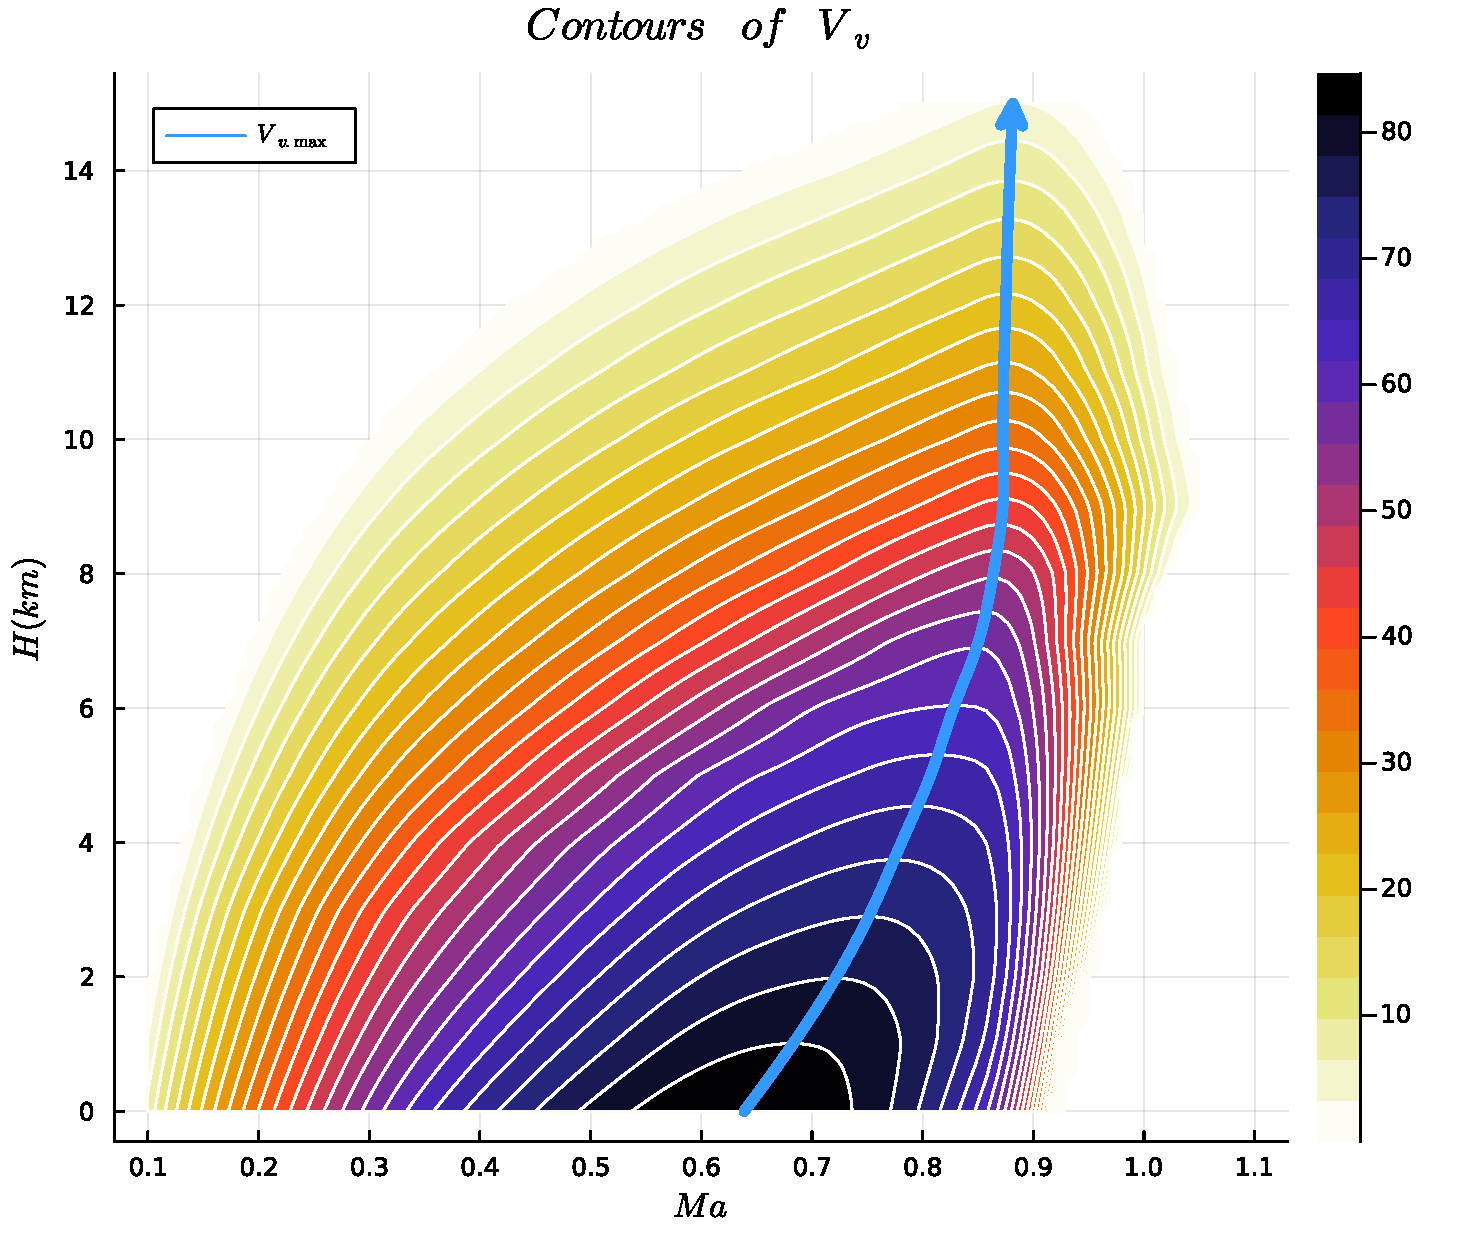
\includegraphics[width=0.5\textwidth]{image/ch5/Contour_Vv.pdf}
    }
    \subfloat[加力状态]{
        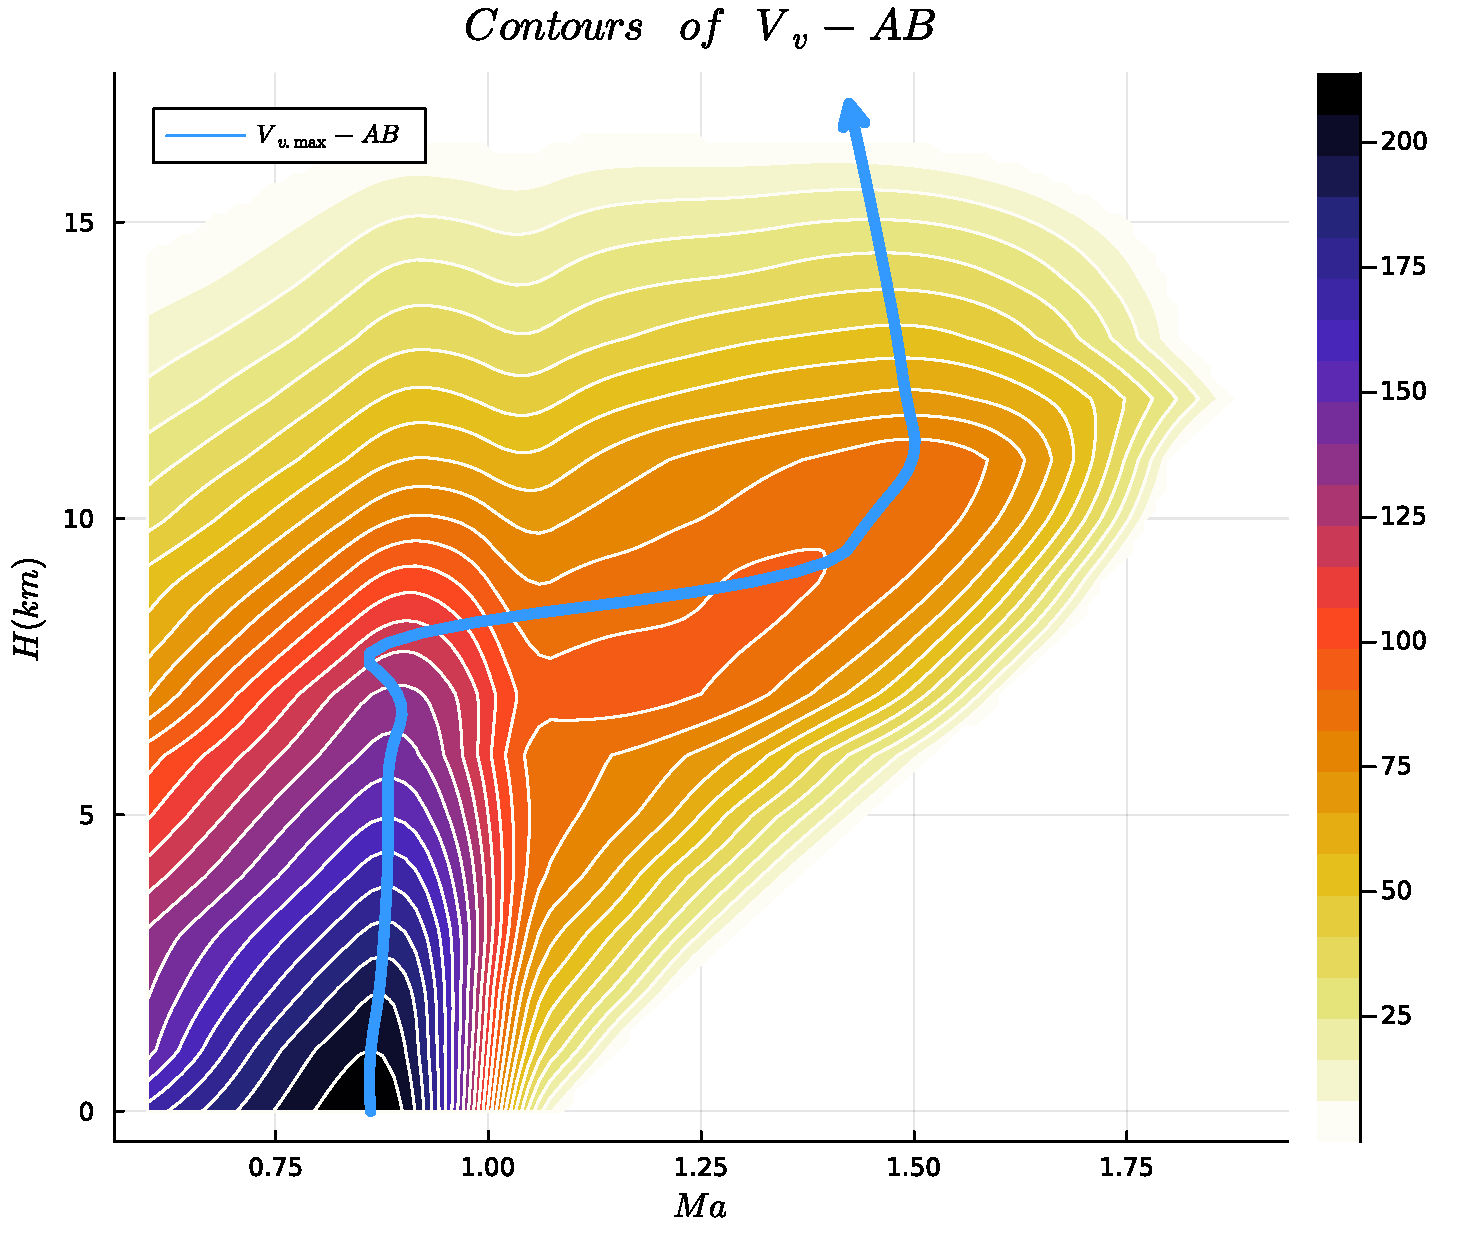
\includegraphics[width=0.5\textwidth]{image/ch5/Contour_VvAB.pdf}
    }
    \caption{单位重量剩余功率SEP云图与最快上升路径示意图}
    \label{单位重量剩余功率SEP云图与最快上升路径示意图}
\end{figure}

在$SEP$也即$V_v$随高度$h$和马赫数$Ma$的关系确定后,
这是一个二元函数关系。
因此在$(h,Ma)$坐标系下,
可以将$SEP$或$V_v$以云图(等值线)的可视化形式表现出来。
如图\ref{单位重量剩余功率SEP云图与最快上升路径示意图}中,
左图为不加力状态,
右图为加力状态。
横坐标为飞行马赫数$Ma$,纵坐标为巡航高度$h$,
云图黑色部分表示最大值,白色表示最小值(如右侧colorbar中所示)。

容易发现$(h,Ma)$的白色边界其实就是飞行包线($\Delta T=0$的边界),
而等值线族的最高点即高度上取得的$V_{v.\max}$。
因此可以将一条“最快上升路径”在该SEP云图中标注出来。
以横坐标$Ma_{qc}$和纵坐标$h^*$为纵坐标,
用蓝色曲线绘制一条最快上升路径。

值得注意的是,
右侧加力状态下,因为高空中$V_{v.\max}$应当取为较快马赫数的$Ma_{qc}$的值,
因此整个曲线会在高空(大致$8km$处)向更快马赫数处“弯折”。


\subsection{上升率所确定的升限}

\begin{figure}[H]
    \centering
    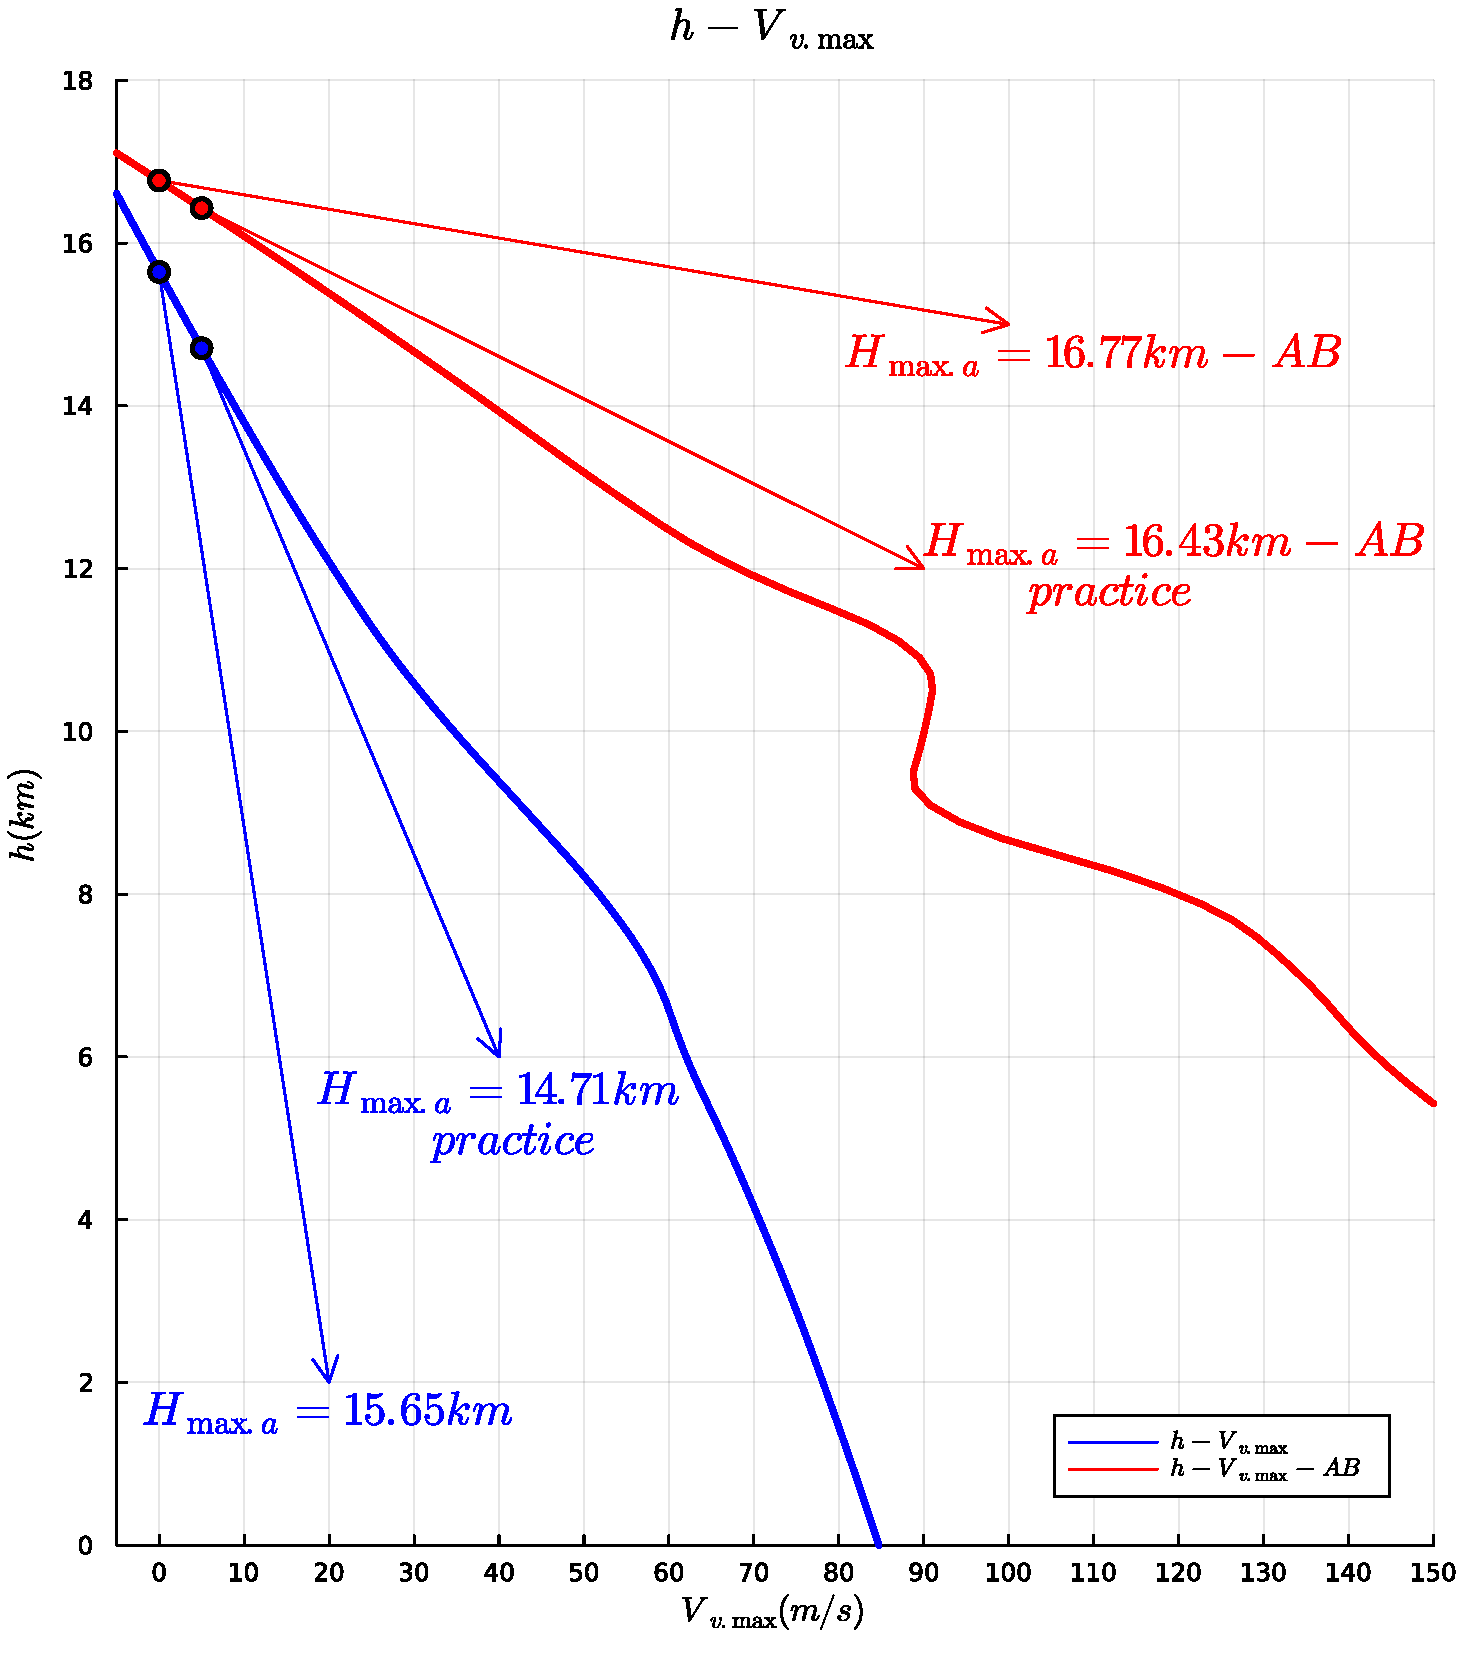
\includegraphics[width=0.6\textwidth]{image/ch5/Vvmax_H.pdf}
    \caption{上升率所确定的升限}
    \label{上升率所确定的升限}
\end{figure}

一般而言认为$V_{v.\max}=0$时的高度就是升限,
因为在此高度上有剩余推力$\Delta T=0$,
没有可以在用于上升的推力,
全部推力用于克服阻力$D$以在此高度上巡航。

将各个高度$h$上的最大上升率$V_{v.\max}$进行绘制曲线,
取$V_{v.\max}=0m/s$的点(即$y$轴交点)可以得到升限,
如图\ref{上升率所确定的升限}所示。
据此思路计算得到的升限为:
\begin{equation}
    \begin{cases}
        \begin{aligned}
            H_{\max .a} & = 15.65km\\
            H_{\max .a} & = 16.77km\quad (AB) 
        \end{aligned}
    \end{cases}
\end{equation}

但因为这个升限需要无穷的时间到达,
因此一般取最大上升率为$V_{v.\max}=5m/s$时的高度$h$为实用(practice)升限。
如图\ref{上升率所确定的升限}中为:
\begin{equation}
    \begin{cases}
        \begin{aligned}
            H_{\max .a} & = 14.71km\\
            H_{\max .a} & = 16.43km\quad (AB) 
        \end{aligned}
    \end{cases}
\end{equation}



\subsection{飞行包线中的快升速度}

在计算得到快升马赫数$Ma_{qc}$后,
可以将其加入飞行包线图,
在一张图中观察各种特征马赫数。

\begin{figure}[H]
    \centering
    \subfloat[$Ma$]{
        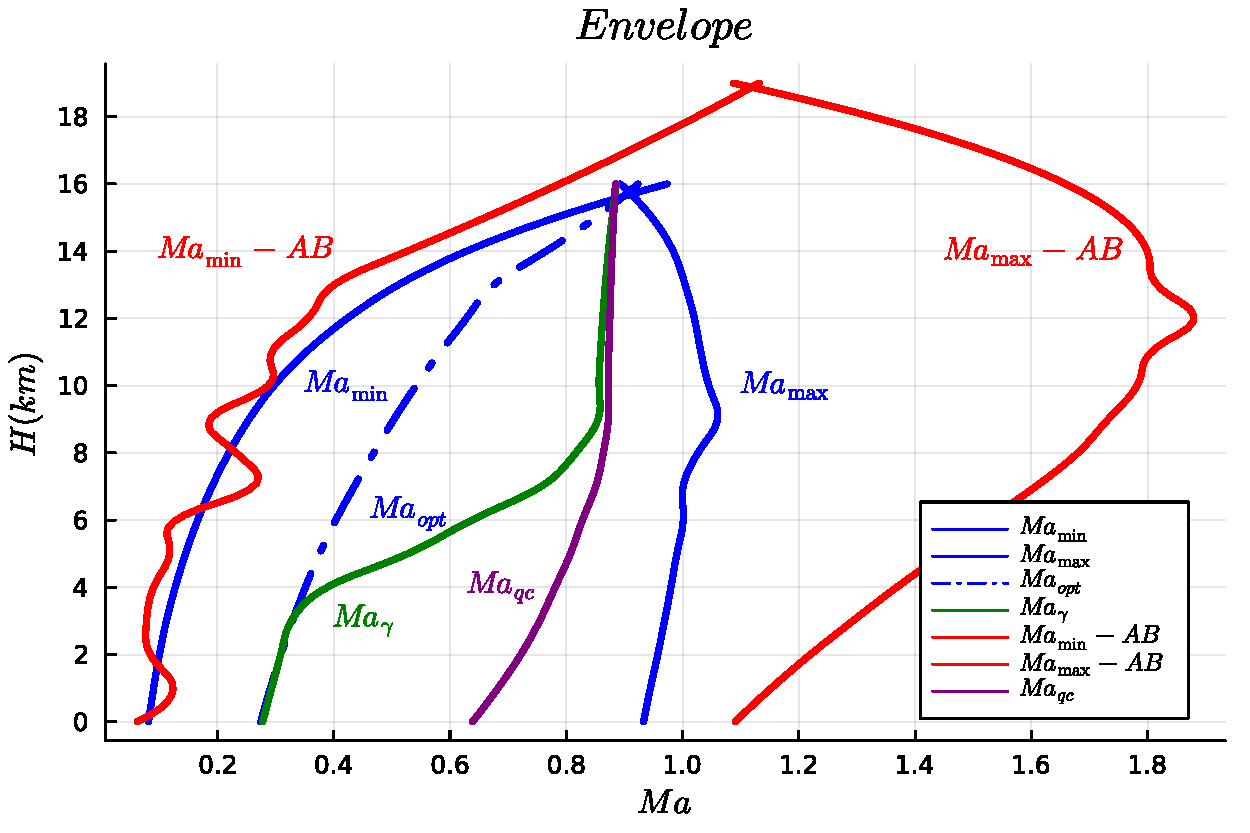
\includegraphics[width=0.5\textwidth]{image/ch5/envelope_qc.pdf}
    }
    \subfloat[$V$]{
        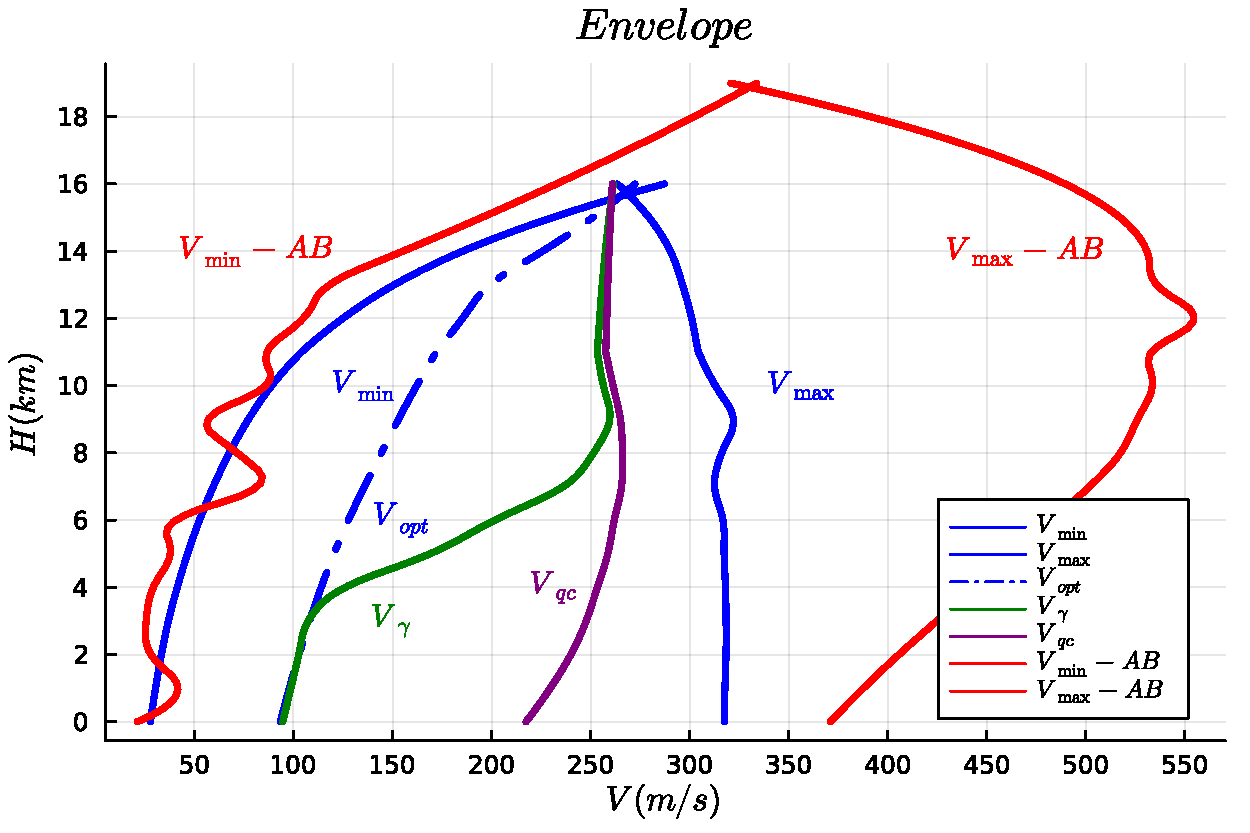
\includegraphics[width=0.5\textwidth]{image/ch5/envelope_V_qc.pdf}
    }
    \caption{加入快升马赫数后的飞行包线}
    \label{加入快升马赫数后的飞行包线}
\end{figure}

容易发现,
在高空中绿色曲线$Ma_{\gamma}$和紫色曲线$Ma_{qc}$在高空中基本重合,
在高空中的陡升马赫数和快升马赫数相一致。
